\documentclass{article}
\usepackage{graphicx}% Required for inserting images
\graphicspath{{./images/}}

%%%%%%%%%%%%%%%%%%%%%%%%%%%%%%%%%%%%%%%%%%%%%%%%%%%%%%%%%%%%%%%%%%%%%%%%%%%%%%%%%%%%%%%%%%%%%%%%%%%%%%%%%%%%%%%%
%%%%%%%%%%%%%%%%%%%%%%%%%%%%%%%%%%%%%%%%%%%%%%%%%%%%%%%%%%%%%%%%%%%%%%%%%%%%%%%%%%%%%%%%%%%%%%%%%%%%%%%%%%%%%%%%
%%%%%%%%%%%%%%%%%%%%%%%%%%%%%%%%%%%%%%%%%%%%%%%%%%%%%%%%%%%%%%%%%%%%%%%%%%%%%%%%%%%%%%%%%%%%%%%%%%%%%%%%%%%%%%%%
% NOTE: We were told in exam that we can't add new packages + exact placement of images isn't important
% Even the pdf generated from this isn't same as ConicSections.pdf but it was given full marks
% Also "1" in "figure 1" in subsection 3.1 Equations is supposed to come using cross-references then only marks were given
%%%%%%%%%%%%%%%%%%%%%%%%%%%%%%%%%%%%%%%%%%%%%%%%%%%%%%%%%%%%%%%%%%%%%%%%%%%%%%%%%%%%%%%%%%%%%%%%%%%%%%%%%%%%%%%%
%%%%%%%%%%%%%%%%%%%%%%%%%%%%%%%%%%%%%%%%%%%%%%%%%%%%%%%%%%%%%%%%%%%%%%%%%%%%%%%%%%%%%%%%%%%%%%%%%%%%%%%%%%%%%%%%
%%%%%%%%%%%%%%%%%%%%%%%%%%%%%%%%%%%%%%%%%%%%%%%%%%%%%%%%%%%%%%%%%%%%%%%%%%%%%%%%%%%%%%%%%%%%%%%%%%%%%%%%%%%%%%%%


\title{Conic Sections}
\author{22b1053}
\date{May 2023}

\begin{document}

% preamble
\maketitle

% below line auto generates the table of contents
\tableofcontents
\clearpage

% section --1
% Introduction section %
\section{Introduction}
% paragraph
A conic section, conic or a quadratic curve is a curve obtained from a cone's surface intersecting a plane. The conic sections in the Euclidean plane have various distinguishing properties, many of which can be used as alternative
definitions.

% section --2
% Types of conic section with lists and figures
\section{Types of Conic Section}
% paragraph
This section explains two types of conic sections.
% unordered list containing figures and content
\begin{itemize}
    \item \textbf{Ellipse}
    \begin{figure}[htbp]
        \centering
        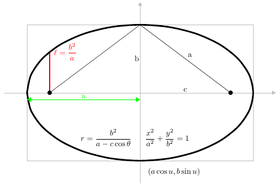
\includegraphics[scale=0.5]{ellipse.png}
        \caption{Ellipse}
        \label{ellipse}
    \end{figure}
    An ellipse is a plane curve surrounding two focal points, such that for all points on the curve, the sum of the two distances to the focal points is a constant
    \item \textbf{Parabola}
    \begin{figure}[htbp]
        \centering
        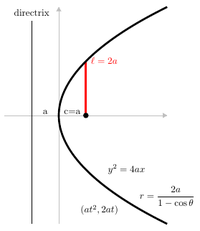
\includegraphics[scale=0.5]{parabola.png}
        \caption{Ellipse}
        \label{parabola}
    \end{figure}
    A parabola is a plane curve which is mirror-symmetrical and is approximately U-shaped.
\end{itemize}

% section --3
% Properties section
\section{Properties}
%paragraph
This section contains the equations for various conic sections and various parameter values.
% Need to use either equation or display math for equations
% subsection --3.1
\subsection{Equations}
% unordered list of equations and content
\begin{itemize}
    \item \textbf{Ellipse} The equation for ellipse in figure \ref{ellipse} is
    \begin{equation}
        \frac{x^{2}}{a^{2}} + \frac{y^{2}}{b^{2}} = 1
    \end{equation}
    \item \textbf{Parabola} The equation for parabola in figure \ref{parabola} is
    \begin{equation}
        y^{2} = 4ax
    \end{equation}
\end{itemize}
% subsection --3.2
\subsection{Parameters}
% tablular code
\begin{table}[htbp]
    \centering
    \begin{tabular}{|c|c|c|}
        \hline
        Conic section type & Eccentricity & Semilatus rectum \\
        \hline
        Ellipse & $\sqrt{1 - \frac{b^{2}}{a^{2}}}$ & $\frac{b^{2}}{a}$ \\
        Parabola & $1$ & $2a$ \\
        \hline 
    \end{tabular}
\end{table}

\end{document}

